% Define the type of document we want to create
\documentclass[paper=a4,media/anfibrief,fromlogo=on]{scrlttr2}

% Packages
\usepackage[utf8]{inputenc}
\usepackage[htt]{hyphenat}
\usepackage{german}
\usepackage{graphicx}
\usepackage{pdfpages}
\usepackage{eurosym}
\usepackage{graphics}
\usepackage{url} % especially useful for line breaks and online version
\PassOptionsToPackage{hyphens}{url} % avoids package loading clash with url and hyperref
\usepackage{hyperref}
\widowpenalty = 10000

\usepackage{fancyhdr}
\fancypagestyle{firststyle}
{
   \fancyhf{}
   \fancyfoot[C]{\tiny Source code available at \, \url{https://github.com/fsi-tue/anfibrief}\\ Latest version available at \, \url{https://teri.fsi.uni-tuebingen.de/anfibrief}\\ Revision: \gitCommit}
   \renewcommand{\headrulewidth}{0pt} % removes horizontal header line
}

% Metadata
\pdfinfo{
  /Author (Fachschaft Informatik)
  /Title  (Brief \studiengang)
  /Subject (\studiengang in Tuebingen)
  /Keywords (Erstsemester;FSI;WSI;Uni Tuebingen,Studienanfaenger;\studiengang)
}

% Beginning of the actual document
\begin{document}
  \date{\today}
  \setkomavar{subject}{\studiengang in T"ubingen }

  \begin{letter}
    {To all first-year students of\\
    \studiengang (\abschluss)\\
    \ifsommersemester
    summer semester \YEAR
    \fi
    \ifwintersemester
    winter semester \YEAR
    \fi
    }

    \opening{Dear newly-enrolled student,}

    we're happy you plan to begin your studies of \studiengang in Tübingen.
To facilitate your start to the studies, we're sending some information to help you get through the first weeks.
You'll receive further tips at our info days.

\textbf{Who or what is this \glqq student council\grqq?} We, the student council of computer science, are a few students from the subjects computer science, bioinformatics, media computer science, cognitive science and medical computer science, who commit themselves to the students' interests. Our work includes on one hand the representation of students in university bodies, on the other hand we try to facilitate the university life of our fellow students (i.e. beginners care,
events, mentoring, and so on).

\ifmaster
    \ifml
We recommend participating at our beginners events, because the transition to master studies or from another university respectively often proves to be difficult. This way you get a first look into everyday life in Tübingen.
    \fi
\fi 
At our events there will be many older students who are willing to answer all your questions. You can find an overview of our events on the following pages.

In case you have questions prior to (or after) our events, you can reach us by mail at \texttt{fsi\At fsi.uni-tuebingen.de}
On our home page
\url{https://www.fsi.uni-tuebingen.de} you can already find helpful information about your studies. If you're interested in collaborating in the student council, just come to one of our meetings. The current date will be published on our web page.

We're looking forward to meeting you at our beginners events!\\
%\vfill
Your student council of computer science
\vfill

\noindent\makebox[\textwidth][c]{%
	\setlength{\fboxrule}{4pt}
	\fcolorbox{green}{white}{
		\begin{minipage}[t]{
				\textwidth}
			If you aren't vaccinated yet, then you can get a vaccination in the special programm of the university.\\
			More information can be found on \url{https://uni-tuebingen.de/universitaet/infos-zum-coronavirus/impfen/}.
\end{minipage}}}

    %\vfill
    %PS: Wir werden aus Datenschutzgründen nicht über die Ablehnungen informiert und schicken diesen
Brief daher grundsätzlich an alle Bewerbenden. Wenn Du Deine Zulassung ablehnen willst, kannst Du diesen Brief
ignorieren -- Du würdest uns allerdings sehr helfen, wenn du uns
kurz per E-Mail über die Gründe für diese Entscheidung informierst.


    \pagebreak
    \Fett{Your schedule for the first days}
    %\Fett{Euer Terminkalender für die ersten Tage}
    \enlargethispage{1ex}
    \setlength{\fboxrule}{4pt}
	\fcolorbox{red}{white}{
		\begin{minipage}[t]{
			\textwidth}\textbf{Achtung!} Aufgrund der aktuellen Lage bezüglich COVID-19 können sich die Anfi-Termine für dieses Semester noch ändern. Wir sind im 				ständigen Austausch mit dem Fachbereich und der Universitätsleitung und müssen den weiteren Verlauf von Verboten und Richtlinien abwarten. 
			Schaut \textbf{auf jeden Fall} immer wieder auf \url{https://www.fsi.uni-tuebingen.de/ersti} nach, dort werden wir die aktuellsten Daten veröffentlichen, 			  sobald wir mehr wissen.
		\end{minipage}}
\begin{description}
  % HINWEIS ZUR ANMELDUNG - GILT IMMER - NICHT LÖSCHEN
  \ifml
    \item[Note:] Unless stated otherwise (i.e. in the description of the event itself), explicitly signing up for the events of the student council is usually \textbf{not necessary}. Details on the respective event can always be found at \url{https://www.fsi.uni-tuebingen.de/ersti} as well.
  \else
    \item[Hinweis:] Sofern nicht anders angegeben (z.B. im Text der jeweiligen Veranstaltung), ist eine explizite Anmeldung zu den Anfi-Veranstaltungen der Fachschaft normalerweise \textbf{nicht nötig}. Weitere Details zur jeweiligen Veranstaltung finden sich auch immer auf \url{https://www.fsi.uni-tuebingen.de/ersti}.
  \fi
  % ENDE HINWEIS ZUR ANMELDUNG

\ifkogwiss
    \ifmaster
        \item[Montag, 30. September \YEAR, 09:00 Uhr, Ort TBA ]\ \\
        Heute beginnt der Vorbereitungskurs Mathematik speziell für Kognitionswissenschaftler im Master. Es ist nicht Pflicht daran teilzunehmen, es ist aber sehr empfehlenswert. Nicht zuletzt lernt ihr hier erste Freunde kennen! Der Vorkurs bietet euch eine Zusammenfassung des Mathestoffs, der im Bachelor Kognitionswissenschaft an der Uni Tübingen behandelt wird.
        \textbf{Wenn ihr euren Bachelor nicht an der Universität Tübingen oder in einem anderen Fach erworben habt, kann der Vorkurs für euch sinnvoll sein.} Falls ihr Quereinsteiger seid, werdet ihr dadurch an die in eurem Studium benötigten mathematischen Grundlagen herangeführt. Falls ihr bereits mathematisches Vorwissen mitbringt, ist der Kurs eine gute Gelegenheit, euer Wissen aufzufrischen.\\
         Es wäre super, wenn ihr euch mit einer kurzen Mail an \texttt{kogni-fachschaft\At fsi.uni-tuebingen.de} bei der Fachschaft Kogni anmelden würdet. Alle weiteren Infos bezüglich Ort und Uhrzeit erhaltet ihr dann von uns.\\

%Stattfinden wird der Vorkurs im ÜR 08 in der alten Physik, das ist die Gmelinstraße 6. Diese befindet sich an der Bushaltestelle Gmelinstraße, nördlich gegenüber von der Neuen Aula. Wenn ihr auf der Wilhelmstraße seid, geht rechts an der Neuen Aula vorbei, dort findet ihr die Alte Physik an der Ecke Gmelin- und Nauklerstraße, rechts von der Neuen Aula. Seid ihr auf der Hölderlinstraße, geht links dran vorbei und die Alte Physik ist auf der linken Straßenseite. Genaue Informationen bezüglich Treffpunkt am ersten Termin erhaltet ihr dann nochmal per Mail.
%
%\seticon{faBus}~\textbf{Bushaltestelle:} Gmelinstraße, Hölderlinstraße, Uni/Neue Aula
%
%\else
    \fi
\fi

\ifml
	\item~ % Funktioniert nicht anders, don't judge me
\else
    \item[Montag, 19. Oktober \YEAR]\ \\
  Heute beginnt der Vorbereitungskurs Mathematik. Es ist nicht Pflicht daran teilzunehmen,
	es ist aber sehr empfehlenswert.
	%Nicht zuletzt lernst du hier erste Freunde kennen!
	\ifsommersemester
	Der Vorkurs bietet dir eine Wiederholung des Schulstoffes sowie eine Übersicht über den Stoff von Mathe II
	\fi
	
	\ifwintersemester
	Der Vorkurs bietet dir eine Wiederholung des Schulstoffes sowie eine Übersicht über den Stoff von Mathe I
	\fi
	
	und führt dich in die Terminologie ein, die du in den Mathe-Vorlesungen wiederfinden wirst.
	
	\ifmaster
	\textbf{Wenn du deinen Bachelor nicht an der Universität Tübingen oder in einem anderen Fach erworben hast, kann der Vorkurs für dich sinnvoll sein. Auf unserer Website findest du ein Skript, von dem ein Teil auch im Vorkurs besprochen wird. Damit solltest du einschätzen können, wie viel vom Stoff bereits bekannt ist und ob sich der Besuch des Vorkurses lohnt.}
	\fi
	
    Um am Vorkurs teilzunehmen, musst du dich bis zum 14. Oktober \YEAR~anmelden. Weitere Informationen erhälst du nach Anmeldung zum Kurs per E-Mail. Falls der Brief aus unerfindlichen Gründen erst nach dem 14. Oktober bei dir eintrifft oder du sonstige Fragen dazu hast, melde dich bitte bei Rüdiger Zell \texttt{ruediger.zeller@uni-tuebingen.de}\\
    \url{https://uni-tuebingen.de/de/91877}.
	% Um Anmeldung wird gebeten, sie ist aber nicht zwingend erforderlich.

	\ifsommersemester
	%Der Vorkurs findet auf dem Gelände des Wilhelm-Schickard-Instituts (oft einfach nur \emph{der Sand} genannt) statt. Du erreichst den Sand per Bus mit den Linien 2 und 6, Haltestelle Sand Drosselweg. Dann ca. 200 Meter Richtung Süden und durch den großen gelben Torbogen. Per Auto erreichst du den Sand über den Nordring (folgt den Schildern "`Uni-Sand"'), hinter dem Hauptgebäude Sand 14 befindet sich ein großer Parkplatz. Der Hörsaal F119 befindet sich jedoch nicht im Hauptgebäude, sondern im Gebäude Sand 6. Nach dem Torbogen direkt links und an den Bäumen entlang, dann stehst du vor dem Haupteingang von Sand 6. Der Hörsaal befindet sich hinter der ersten Tür links.
	%Bitte beachtet, dass das Semesterticket \emph{erst ab dem 1.4} gültig ist. Falls du davor Tübingen schon unsicher machst und Bus fahren willst, musst du dir extra Fahrscheine kaufen.
	%Natürlich kommt man zur Morgenstelle auch zu Fuß oder mit dem Rad, da es jedoch steil den Berg hochgeht, muss man hierfür einiges an Zeit einrechnen.
	\fi

	%\seticon{faBus}~\textbf{Bushaltestelle:} Linie 2, Linie 6 "`Sand Drosselweg"' (Rest ausgeschildert)
\fi

\ifmaster
    \ifbinfo
        \item[Mittwoch, 21. Oktober \YEAR, TBA, Sand]\ \\
            Heute beginnt ein Informatik-Vorkurs speziell für Bioinformatik-Studenten im Master. Dieser Vorkurs wird dringend empfohlen, wenn du aus einem fachfremden Studiengang wie z.B. Biologie oder anderen Lebenswissenschaften kommst und noch keine oder sehr wenig Erfahrung in der Informatik und der Programmierung (CLI, Java, Python, \LaTeX) hast. Der Vorkurs wird in Englisch gehalten. Anmeldeschluss ist bis zum 20. Oktober, 12 Uhr. Alle weitere Informationen und die Anmeldung findest du auf folgender Website: \\ \url{https://uni-tuebingen.de/de/91881}

        \seticon{faBus}~\textbf{Bushaltestelle:} Linie 2, Linie 6 Sand Drosselweg
    \fi
\fi

\ifbachelor
    \iflehramt
        \item[Dienstag, 3. November \YEAR, TBA]\ \\
            Deine erste Vorlesung beginnt. \\
            Du hast um 14 Uhr „Informatik I“ bei \Infoprof.
            Alles, was du heute (und in Zukunft) benötigst: persönlichen Wachmacher, einen Stift, einen Block und den Studierendenausweis.

            %\seticon{faBus}~\textbf{Bushaltestelle:} BG Unfallklinik (Linie 5, 13, 14, 17, 18, 19, X15)
    \else
        \item[Montag, 2. November \YEAR, TBA]\ \\
            Deine erste Vorlesung beginnt. \\
            Du hast um 8 Uhr „Mathematik I“ bei \Matheprof.
            Alles, was du heute (und in Zukunft) benötigst: persönlichen Wachmacher, einen Stift, einen Block und den Studierendenausweis.

            %\seticon{faBus}~\textbf{Bushaltestelle:} BG Unfallklinik (Linie 5, 13, 14, 17, 18, 19, X15)
    \fi
\fi

%Spieleabend 1
%\ifml
%	\item[Friday, October 4th, \YEAR, 19:00, Sand]\ \\
%	We'd like to invite you to (an analog) board game evening with relaxed atmosphere at the Sand. We'll provide some games as well as drinks and snacks (for a small donation). Even though our collection is growing steadily, we're more than happy if you bring along your own games! Further details will be provided at \url{https://www.fsi.uni-tuebingen.de/ersti}.

%	\seticon{faBus}~\textbf{bus stop:} route 2, route 6 "`Sand Drosselweg"' (signposted from there)
%\else
%    \item[Donnerstag, 23. April \YEAR, 18:00 Uhr, Sand 1 A301]\ \\
%	Wir möchten dich zu einem kleinen (analog-) Spieleabend mit guter Gesellschaft und entspannter Atmosphäre auf dem Sand einladen. Für einige Spiele sowie Getränke und Knabberkram (gegen einen kleinen Obolus) sorgt die Fachschaft. Wir freuen uns natürlich sehr, wenn du auch eigene Spiele mitbringst, obwohl unsere Sammlung schon beachtlich ist! Details werden noch auf \url{https://www.fsi.uni-tuebingen.de/ersti/} bekannt gegeben.

%	\seticon{faBus}~\textbf{Bushaltestelle:} Linie 2, Linie 6, Sand Drosselweg (Rest ausgeschildert)
%\fi

%Filmabend
%\ifml
%	\item[Tuesday, October 2nd, \YEAR, 19:00, Sand 14, room A104 (meeting point is signposted)]\ \\
%	On this evening still early into the semester, we would like to invite you to a cozy movie night at the Sand. This is a perfect opportunity to relax, get to know the Sand, meet the people of the student council and future co-eds while watching a movie \footnote{Due to license restrictions, we're not allowed to tell you what movie wil be shown}.

%	\seticon{faBus}~\textbf{bus stop:} route 2, route 6 "`Sand Drosselweg"' (signposted from there)
%\else
	%\item[Dienstag, 31. März \YEAR, 19:00 Uhr, Sand 1 A301]\ \\
    %Am Abend des zweiten Vorkurstages möchten wir dich zu einem gemütlichen Filmabend auf dem Sand einladen.
	%Hier hast du die Möglichkeit, bei einem Film \footnote{welcher Film gezeigt wird, dürfen wir aus lizenzrechtlichen Gründen nicht bekannt geben.} zu entspannen, einige Fachschaftler, den Sand und eure zukünftigen Kommilitonen kennen zu lernen.

	%\seticon{faBus}~\textbf{Bushaltestelle:} Linie 2, Linie 6, Sand Drosselweg (Rest ausgeschildert)
%\fi

% Bus-Schnitzeljagd, neu im WS19/20
%\ifml
%	\item[Monday, October 7th \YEAR, 19:00, \textbf{in front of} Neckarmüller]\ \\
%    During a scavenger hunt you will be sent off in teams to explore the Tübingen bus network. By solving various puzzles, you will not only get to know your new fellow students better, but also get to know some stops that you will encounter more or less frequently in your everyday university life. Since students in Tübingen (and in the complete naldo area) are allowed to take the bus and train free of charge from Monday to Friday from 19:00 \footnote{as well as all day on Saturdays, Sundays and public holidays in Baden-Württemberg} onwards, you only need your student ID card for your exploration tour.\\
%If details change, you will find further information such as time and meeting point on our website \url{https://www.fsi.uni-tuebingen.de/ersti/}.\\

%\else
%	\item[Montag, 7. Oktober \YEAR, 19:00 Uhr, vor dem Neckarmüller]\ \\
%    Bei der Schnitzeljagd wirst du mit deinen Kommilitonen in Teams losgeschickt, um das Tübinger Busnetz zu erkunden. Durch das Lösen verschiedener Rätsel lernt ihr dabei nicht nur eure neuen Komilitonen sondern auch einige Haltestellen besser kennen, die euch in eurem Uni-Alltag mehr oder weniger häufig begegnen werden. Da Studenten in Tübingen (und im kompletten naldo-Bereich) montags bis freitags ab 19:00 Uhr \footnote{sowie ganztägig an Samstagen, Sonntagen und gesetzlichen Feiertagen in Baden-Württemberg} kostenlos Bus und Bahn fahren dürfen, benötigt ihr für eure Erkundungstour lediglich euren Studierendenausweis.\\
%    Falls sich Details ändern sollten, findest du weitere Infos wie Uhrzeit und Treffpunkt auf unserer Webseite \url{https://www.fsi.uni-tuebingen.de/ersti}.\\
%\fi

%Grillen
%\ifml
%	\item[Tuesday, October 15th \YEAR, 17:00, Sand 13, garden]\ \\
%	You're not in the mood for cooking this evening? Fear not! The student coucil invites you for a BBQ. Bring whatever you want to put on the grill, please also bring your own plates and cutlery. The garden has enough space for stuff like volleyball, football etc. as well.
%	If the schedule should change somehow, you can find updated details on our website at \url{https://www.fsi.uni-tuebingen.de/ersti/}.

%	\seticon{faBus}~\textbf{bus stop:} route 2, route 6, "`Sand Drosselweg"' (signposted from there)
%\else
	%\item[Donnerstag, 2. April \YEAR, 18:00 Uhr, im Garten des Sandes ]\ \\
	%Du hast keinen Bock auf Kochen? Dann bist du hier genau richtig! In geselliger Runde wird die Fachschaft mit dir grillen. Bringt dazu mit, was auch immer du zum Grillen brauchst, Gas- und Kohlegrill warten auf dich. Bring bitte auch dein Besteck und Geschirr selbst mit!\\
	 %Auf dem Sand ist es auch möglich, Volleyball, Fußball, usw. zu spielen. Wir freuen uns auf dich!
	%Falls sich Details ändern sollten, findest du weitere Infos wie Uhrzeit und Treffpunkt auf unserer Webseite \url{https://www.fsi.uni-tuebingen.de/ersti/}.

	%\seticon{faBus}~\textbf{Bushaltestelle:} Linie 2, Linie 6, Sand Drosselweg (Rest ausgeschildert)
%\fi

%Stadtrallye
\ifml
	\item[Saturday, October 24th \YEAR, 16:00 Uhr, \textbf{in front of} Neckarmüller ]\ \\
	On this evening, you can participate in a team-based scavenger hunt across the city, where you will get to know interesting, beautiful as well as disturbing spots within Tübingen. As a side effect, you will hopefully get to know your new home town a bit better and make new friends. The meeting point is at the Neckarbrücke \emph{in front of the} restaurant "`Neckarmüller"`.
	If the schedule (time and meeting point) should change somehow, you will find the new details on our website at \url{https://www.fsi.uni-tuebingen.de/ersti/}.

	\seticon{faBus}~\textbf{bus stop:} route 2, "`Sand Drosselweg"' (signposted from there)
\else
	 \item[Samstag, 24. Oktober \YEAR, 16:00 Uhr, \textbf{vor} dem Neckarmüller ]\ \\
	 Bei der Stadtrallye lassen wir dich und deine Kommilitonen gegeneinander in Teams antreten. Dabei werdet ihr interessante, schöne und verstörende Ecken Tübingens kennen lernen, dabei hoffentlich die Orientierung in eurer neuen Heimat etwas verbessern und Kontakte knüpfen. Der Treffpunkt ist bei der Neckarbrücke (\emph{vor} dem Gasthaus „Neckarmüller“).
	 Falls sich Details ändern sollten, findest du weitere Infos wie Uhrzeit und Treffpunkt auf unserer Webseite \url{https://www.fsi.uni-tuebingen.de/ersti/}.
\fi

%Online Stadtrallye
%\item[Dienstag, 1. November \YEAR, TBA]\ \\
%	 Dieses Semester ist die erste Online Stadtrallye geplant. Kommt vorbei und lernt die Stadt kennen.

% Frühstück
%\ifml
% Frühstück Master ML
%    \item[Friday, October 11th \YEAR, 9:00, Mensa Morgenstelle]\ \\
%        Let's have breakfast together, we're paying! You will get to know a lot of stuff about the university, the student council, what it's like to study in Tübingen and what you can expect in the upcoming months -- especially when talking to older co-eds.
%    \ifwintersemester You will also be greeted by \Infoprof~-- he will lecture Informatics I. This is a lecture for bachelor students, but maybe you will get to know him in other lectures as well. \fi
%    Afterwards, we will provide a tour of the Morgenstelle so you get to know the most important rooms and lecture halls.
%    You can reach the Morgenstelle via bus, bicycle or on foot. However, the way up to the Morgenstelle is quite steep -- Tübingen is hilly (German: \emph{hügelig}), so you should factor in the time you need to get there.
%    The simplest (but also steepest) way is via "`Parkhaus König"' and up "`Schnarrenbergstraße"', past the university hospital. If you're starting at Waldhäuser Ost, follow the "`Nordring"' in direction of "`Uni-Morgenstelle"' / "`Kliniken Berg"'.
%    If you want to drive there by car, you can park (not free!) by the side of the road on Nordring or inside the multi-story cark park "`Ebenhalde"' north of the Morgenstelle. However, the simplest way is via bus.
%    From 11:45 onwards, you can try out the mensa food if you like.\\
%    \seticon{faBus}~\textbf{bus stop:} BG Unfallklinik (bus routes 5, 13, 14, 17, 18, 19, X15)

%\else
    %\item[Donnerstag, 9. April \YEAR, 9:00 Uhr, Sand 1 A104]\ \\
        %Wir laden dich an diesem Morgen zu einem gemütlichen Frühstück ein! Dabei erfährst du einiges über die Uni, die Fachschaft und was dich in den nächsten Monaten erwartet -- auch im Gespräch mit älteren Studierenden.
%    \ifwintersemester Außerdem wirst du durch \Infoprof~-- er wird die Informatik I Vorlesung halten -- begrüßt. \fi
    %\ifsommersemester Außerdem wirst du durch \Infoprof~-- er wird die Informatik II Vorlesung halten -- begrüßt. \fi
    %\ifmaster Zwar ist Informatik I eine Bachelor-Veranstaltung, aber du wirst \Infoprof~ vielleicht auch in Master-Vorlesungen kennen lernen. \fi
%    \ifwintersemester
%        Danach machen wir eine Führung über die Morgenstelle, damit du die wichtigsten Räume und Hörsäle kennen lernst.
%        Zur Morgenstelle kommt man entweder mit dem Bus, zu Fuß oder mit dem Rad. Da der Weg zur Morgenstelle aber sehr steil ist (Tübingen ist hügelig), sollte man hierfür einiges an Zeit einrechnen.
%        Der einfachste Weg ist hier über das Parkhaus König. Von dort musst du bergauf der Schnarrenbergstraße folgen. Es geht dann zunächst an den Uni-Kliniken Berg vorbei, anschließend erreichst du die Morgenstelle. Falls du aus der Richtung Waldh\"auser-Ost kommt, so musst du dem Nordring in Richtung Kliniken Berg folgen. Für beide Wege solltest du jeweils mindestens eine halbe Stunde zu Fuß einrechnen.
%        Wenn du mit dem Auto ankommst, kannst du (kostenpflichtig) an den Straßenseiten des Nordrings, oder im Parkhaus "`Ebenhalde"' oberhalb der Morgenstelle parken. Am einfachsten geht es jedoch mit dem Bus.
%        Wenn du Lust hast, kannst du ab 11:45 Uhr das Mensaessen ausprobieren.
%    \fi

%    \ifwintersemester \seticon{faBus}~\textbf{Bushaltestelle:} BG Unfallklinik (Linie 5, 13, 14, 17, 18, 19, X15) \fi
    %\ifsommersemester \seticon{faBus}~\textbf{Bushaltestelle:} Linie 2, Linie 6, Sand Drosselweg \fi
%\fi

\iflehramt
    \ifbachelor
        %\item[Donnerstag, 9. April \YEAR, 10:00-12:00 Uhr, Kupferbau, Hörsaal 22]\ \\
            %Anfis im \textbf{Bachelor of Education} können beim Frühstück (rein theoretisch) nicht mit dabei sein, denn parallel zum Frühstück werdert ihr um 10:00 Uhr über die speziellen Anforderungen des Lehramtsstudiums informiert. Neben den eigentlichen Fachinhalten kommen im Bachelor of Education noch einige andere Dinge auf euch zu, z.B. ein Orientierungspraktikum, die Fachdidaktik und der Studienbereich Bildungswissenschaften. Zu Beginn des Masters steht dann ein Schulpraxissemester an, und nach dem Studienabschluss das Referendariat. Bei dieser Veranstaltung werden euch alle diese Elemente des Lehramtsstudiums vorgestellt.

        %\seticon{faBus}~\textbf{Bushaltestelle:} Hölderlinstraße bzw. Uni/Neue Aula
    \fi
    \ifmaster
        %\item[Donnerstag, 9. April \YEAR, 14:00-16:00 Uhr, Kupferbau, Hörsaal 22]\ \\
            %Wenn du im \textbf{Master of Education} studierst, kannst du zum Frühstück bleiben, eure Einführungsveranstaltung beginnt dann erst um 14 Uhr. Hier bekommst du u.a. einen Einblick in die verschiedenen Studienanteile des Master of Education und Informationen zum Schulpraxissemester.
    \fi
\fi
%Begrüßung Online
\item[Freitag, 30 Oktober \YEAR, 10:00 Uhr, via Zoom]
An diesem Tag werdet ihr von den Professoren aus unserem Fachbereich begrüßt. Nähere Details folgen.
% Kneipentour
\ifml
	\item[Friday, October 30th \YEAR, 18:00, \textbf{in front of} Neckarmüller]\ \\
        Tübingen is laced with small bars and pubs that have a significant impact on the night life in Tübingen. In order to calm down from the stress of this information-filled day, we'd like to invite you to go bar-hopping with us. We'll divide up into small groups and visit the different bars in the historic town center. Please bring enough cash, most places we will visit don't accept cards (\emph{none whatsoever}).

	\else
	\item[Samstag, 14. November \YEAR, 19:00 Uhr, \textbf{vor} dem Neckarmüller]\ \\
        Tübingen ist übersät mit kleinen Kneipen und Bars, die das Nachtleben maßgeblich beeinflussen. Um den Stress des informationsgefüllten Tages etwas sacken zu lassen, laden wir dich zu einer ausgiebigen Kneipentour ein, bei der wir in Kleingruppen die verschiedenen Lokalitäten der Tübinger Altstadt besuchen. Bitte bringe genügend Bargeld mit, man kann in fast keiner der Tübinger Bars mit EC-Karte zahlen! -- Volksbanken und Sparkassen finden sich bei Bedarf in der Stadt.
\fi

\ifwintersemester
    \ifml
	    \item[Friday, October 11th, \YEAR, 14:00, Sand, Foyer (rooms and schedule will follow)]\ \\
    	At 2 o'clock, we'll meet up again at the Sand, home of the faculty of computer science. % Ich weiß dass es keine Fakultät ist, übersetz mir mal einer Fachbereich...
    	Here you can gain some interesting insights into the work of the different work groups present at the Sand.
	    Getting to know the work groups makes sense for ML as well, depending on how you want to focus your studies or thesis. Depending on your interests you can participate in different mini workshops or listen to talks, however, this requires some planning on your part. The talks available (as well as the time slots) are subject to change, please refer to \url{https://www.fsi.uni-tuebingen.de/ersti/} the day before.
    	For the most part, the work groups focusing on Machine Learning are located at the Tübinen AI research building, however, access there is rather restricted.

	    \seticon{faBus}~\textbf{bus stop:} route 2, route 6, "`Sand Drosselweg"' (signposted from there)
    \else
	    \item[Freitag, 11. Oktober \YEAR, 14 Uhr, Sand 1, Foyer (Räume und Programm folgen)]\ \\
    	Um 14:00 treffen wir uns auf dem Sand (dem Sitz der Informatik in Tübingen) wieder. Hier werden wir dich mit Informationen rund um das Studium und die Arbeit unserer Lehrstühle auf dem Sand versorgen.
    	Nachdem du über den Verlauf des Studiums der ersten Wochen, Monate und Semester informiert wurdest, bieten dir die verschiedenen Fachbereiche mit interaktiven Vorträgen einen Einblick in ihre Arbeit. Die Fachbereiche kennen zu lernen lohnt sich für Studierende aller Studiengänge. Die Vorträge zeigen, welche Themen am Wilhelm-Schickard-Institut verfolgt werden, geben dir ein Gefühl, was für dich hier interessant sein kann und wo du möglicherweise Schwerpunkte im Studium, einer Studien- oder Abschlussarbeit setzen willst. Je nach Interesse kannst du dir verschiedene Vorträge anhören, allerdings bedarf dies an Auswahl und Planung von deiner Seite. Die angebotenen Vorträge können sich thematisch oder, wie die Begrüßungen, im Zeitrahmen ändern. Schau daher auch kurzfristig (am selben Tag) auf \url{https://www.fsi.uni-tuebingen.de/ersti/} nach.

        \seticon{faBus}~\textbf{Bushaltestelle:} Linie 2, Linie 6, Sand Drosselweg (Rest ausgeschildert)
    \fi
\fi

%Mastercafé
\ifmaster
    \ifml
        \item[Friday, October 11th \YEAR, 11:00, Maria-von-Linden-Straße 6]\ \\
    At this informal meeting you will have the opportunity to get to know your fellow students and some of the lecturers over a coffee. And then there will be cake.\footnote{This is not a lie!}

        \seticon{faBus}~\textbf{bus stop:} route 3, "`Maria-von-Linden-Straße"' (signposted from there)
    \else
    %\item[Dienstag, 14. März \YEAR, 16:00 Uhr, Sand 1 A301]\ \\
    %Bei diesem informellen Treffen hast du Gelegenheit, neue Master-Studierende aus deinem eigenen und auch aus anderen Studiengängen sowie einige der Dozenten bei Kaffee kennenzulernen. Und dann gibt es Kuchen. \footnote{Das ist keine Lüge!}

        %\seticon{faBus}~\textbf{Bushaltestelle:} Linie 2, Linie 6, Sand Drosselweg (Rest ausgeschildert)
    \fi
\fi

%Um 13{\ifkogwiss}:45{\fi} Uhr treffen wir uns auf dem „Sand“ (dem Sitz des Wilhelm-Schickard-Instituts)
%wieder. Hier werden wir euch mit Informationen rund um{\ifkogwiss} {\else} euer Studium und {\fi}die Arbeit unserer Lehrstühle auf dem Sand versorgen.
%
%{\ifkogwiss}Als Studierende der Kognitionswissenschaften könnt ihr um 13:45 Uhr zusto{\ss}en, die anderen Studiengänge erhalten vorab eine spezifische Einführung, die für euch Montag, 15. Oktober am Psychologischen Institut stattfindet. {\else}{\ifinfo}Als Lehramt Informatik und Informatik-Studierende werden euch auch mögliche Nebenfächer vorgestellt, ihr werdet {\else}Ihr werdet als *-Informatik-Studierende {\fi}noch einmal spezifisch begrüßt und ihr erhaltet einen studiengangsspezifischen Einblick in Forschung und Lehre.{\fi}
%
%{\ifkogwiss}Die {\else}Nachdem ihr über den Verlauf des Studiums der ersten Wochen, Monate und Semester informiert wurdet, bieten euch die {\fi}verschiedenen Fachbereiche {\ifkogwiss}auf dem Sand bieten euch {\else} {\fi}mit Vorträgen einen Einblick in ihre Arbeit. Die Fachbereiche kennen zu lernen lohnt sich für Studierende aller Studiengänge, die Vorträge zeigen welche Themen am Wilhelm-Schickard-Institut verfolgt werden, geben euch ein Gefühl, was für euch hier interessant sein kann und wo ihr möglicherweise Schwerpunkte im Studium, einer Studien- oder Abschlussarbeit setzten wollt. Je nach Interesse könnt ihr euch verschiedene Vorträge anhören, allerdings bedarf dies an Auswahl und Planung von eurer Seite. Die angebotenen Vorträge können sich thematisch oder, wie die Begrüßungen, im Zeitrahmen ändern. Schaut daher auch kurzfristig (am selben Tag) auf \url{https://www.fsi.uni-tuebingen.de/ersti/} nach.
%
%\seticon{faBus}~\textbf{Bushaltestelle:} Sand Drosselweg (Rest ausgeschildert)


%\item[Freitag, 12. Oktober \YEAR, 13{\ifkogwiss}:45{\fi} Uhr, Sand (Räume und Programm folgen)]\ \\
%Um 13{\ifkogwiss}:45{\fi} Uhr treffen wir uns auf dem „Sand“ (dem Sitz des Wilhelm-Schickard-Instituts)
%wieder. Hier werden wir euch mit Informationen rund um{\ifkogwiss} {\else} euer Studium und {\fi}die Arbeit unserer Lehrstühle auf dem Sand versorgen.
%
%{\ifkogwiss}Als Studierende der Kognitionswissenschaften könnt ihr um 13:45 Uhr zusto{\ss}en, die anderen Studiengänge erhalten vorab eine spezifische Einführung, die für euch Montag, 15. Oktober am Psychologischen Institut stattfindet. {\else}{\ifinfo}Als Lehramt Informatik und Informatik-Studierende werden euch auch mögliche Nebenfächer vorgestellt, ihr werdet {\else}Ihr werdet als *-Informatik-Studierende {\fi}noch einmal spezifisch begrüßt und ihr erhaltet einen studiengangsspezifischen Einblick in Forschung und Lehre.{\fi}
%
%{\ifkogwiss}Die {\else}Nachdem ihr über den Verlauf des Studiums der ersten Wochen, Monate und Semester informiert wurdet, bieten euch die {\fi}verschiedenen Fachbereiche {\ifkogwiss}auf dem Sand bieten euch {\else} {\fi}mit Vorträgen einen Einblick in ihre Arbeit. Die Fachbereiche kennen zu lernen lohnt sich für Studierende aller Studiengänge, die Vorträge zeigen welche Themen am Wilhelm-Schickard-Institut verfolgt werden, geben euch ein Gefühl, was für euch hier interessant sein kann und wo ihr möglicherweise Schwerpunkte im Studium, einer Studien- oder Abschlussarbeit setzten wollt. Je nach Interesse könnt ihr euch verschiedene Vorträge anhören, allerdings bedarf dies an Auswahl und Planung von eurer Seite. Die angebotenen Vorträge können sich thematisch oder, wie die Begrüßungen, im Zeitrahmen ändern. Schaut daher auch kurzfristig (am selben Tag) auf \url{https://www.fsi.uni-tuebingen.de/ersti/} nach.
%
%\seticon{faBus}~\textbf{Bushaltestelle:} Sand Drosselweg (Rest ausgeschildert)

% erste Vorlesung
%\ifbachelor
%\item[Dienstag, 14. April \YEAR, Morgenstelle, Hörsaal N7]\ \\
%Deine erste Vorlesung beginnt um
%\ifwintersemester 8 Uhr -- Du hast „Mathe I für Informatiker“  \fi
%\ifsommersemester 10 Uhr -- Du hast „Mathe II für Informatiker“  \fi
%bei \Matheprof.
%Alles, was du heute (und in Zukunft) benötigst: persönlichen Wachmacher, einen Stift, einen Block und den Studierendenausweis.

%\seticon{faBus}~\textbf{Bushaltestelle:} BG Unfallklinik (Linie 5, 13, 14, 17, 18, 19, X15)
%\fi

%Akadem. Spieleabend
%\ifml
%    \item[Thursday, October 17th, \YEAR 18:00 Sand 1, A301]\ \\
%        On this afternoon/evening we'd first like to invite you a second time to play board games with your fellow students. As soon as the time has advanced far enough, we'd like to live it up in the pubs.\\
%	\seticon{faBus}~\textbf{bus stop:} route 2, route 6 "`Sand Drosselweg"' (signposted from there)
%\else
    %\item[Donnerstag, 16. April \YEAR, 19:00 Uhr, Sand 1 A301]\ \\
%An diesem Nachmittag/Abend möchten wir dich zunächst auf den Sand einladen, um in gemütlicher Runde mit anderen Kommilitonen und Fachschaftlern Brett- und Gesellschaftsspiele zu spielen. Sobald die Zeit an diesem Abend ausreichend fortgeschritten ist, möchten wir zusammen mit dir ein wenig die Kneipen der Altstadt unsicher machen.

%\seticon{faBus}~\textbf{Bushaltestelle:} Linie 2, Linie 6, Sand Drosselweg (Rest ausgeschildert)
%\fi

%Online Spieleabend
\item[Freitag, 30. Oktober]
	Heute findet das speziell unter Corona-Bedingungen eingeführte Online-Spieleabend der Fachschaft statt. Wir organisieren eine Kommunikationsmöglichkeit über Discord und viele Spiele wie Drawful2,.....usw.
	
%\item[Freitag, 6. November]
%	Heute findet der zweite Online-Spieleabend der Fachschaft statt. yWir organisieren eine Kommunikationsmöglichkeit über Discord und viele Spiele wie Drawful2,.....usw.


%TODO Text Wanderung
\item[Sonntag, 25. Oktober, \YEAR 11 Uhr, Neckarmüller; Sonntag, 08. November, \YEAR 11 Uhr, WHO (Waldhäuserstraße 122, 72076 Tübingen)]\ \\
        Bei einer gemütlichen Wanderung lernt ihr neben euren Kommilitonen und Kommilitoninnen auch noch die sehenswerte Tübinger Umgebung kennen! Für genauere Informationen schaut nochmals in den Kalender der Fachschaft Info und das dazugehörige Google Doc.\\
	\seticon{faBus}~\textbf{bus stop:} Linie 2, 3, 4, 5 "Ulmenweg", WHO

\ifkogwiss
\item[Montag, 14. Oktober \YEAR, Uhrzeit und Ort TBA]\ \\
    Hier stellen sich die kognitionswissenschaftlichen Lehrstühle (also die verschiedenen Forschungsbereiche der Professoren) vor. Dies ist super um einen Überblick zu bekommen, was die Kognitionswissenschaft alles beinhaltet und um erste Eindrücke von den Profs zu bekommen. Auch die Fachschaft stellt sich dir hier erstmals vor. Danach gibt es noch Gelegenheit, mit der Fachschaft ein Glas Milch trinken zu gehen. Auch für Kogni-Master ist das eine super Veranstaltung.
\fi

\ifkogwiss
    \item[Mittwoch, 16. Oktober, \YEAR, Uhrzeit und Ort TBA]\ \\
         Damit man sich auch unter den Kognis kennenlernen kann, veranstalten wir einen Spiele- und Informationsabend für die Kogni-Anfis. Hier können Gesellschaftsspiele und bei gutem Wetter auch Tischtennis und Volleyball gespielt werden. Für Verpflegung können wir leider nicht auf eigene Kosten sorgen aber wir stellen gegen eine kleine Spende Getränke bereit und bestellen Pizza. Es werden auch einige höhersemestrige Kognis und Fachschaftler da sein, die man zum Kogni-Studium ausfragen kann. Kogni-Master sind natürlich auch herzlich eingeladen.
	\seticon{faBus}~\textbf{Bushaltestelle:} Linie 2, Sand Drosselweg (Rest ausgeschildert)
\fi

%Clubhausfest
\ifml
    \item[Thursday, January 14th, \YEAR, 18:00, Clubhaus]\ \\
        Every Thursday during the lecture period, a different student body or group of students organizes the "`Clubhaus Fest"'\footnote{a university building where a different student council hosts a party every thursday} in the Clubhaus, directly opposite the New auditorium. Today the attendance is particularly worthwhile, because the student councils of computer science, cognitive science and psychology are hosts! We are looking forward to meeting you!(This event is scheduled to take place, but the circumstances may still change because of the corona virus!)

        \seticon{faBus}~\textbf{bus stop:} Uni/Neue Aula or Hölderlinstraße
\else
    \item[Donnerstag, 14. Januar \YEAR, 21:00 Uhr, Clubhaus ]\ \\
        Während der Vorlesungszeit richtet jeden Donnerstag eine andere Fachschaft oder studentische Gruppierung das Clubhausfest im Clubhaus, direkt gegenüber der Neuen Aula, aus. Heute lohnt sich der Besuch jedoch ganz besonders, denn die Fachschaften Informatik, Kogni und Psychologie sind Gastgeber! Wir freuen uns auf dich! (Dieses Ereignis findet vorraussichtlich statt, jedoch kann sich die Situation wegen Corona immer noch ändern!)
%Das anfängliche Chaos des Vorlesungsbeginns hat sich gelegt und auch an diesem Donnerstag findet das Clubhausfest statt.

%\seticon{faBus}~\textbf{Bushaltestelle:} Uni/Neue Aula bzw. Hölderlinstraße
\fi

%Anfiwochenende
%\ifml
%    \item[Friday, October 18th, \YEAR, 13:00, train station]\ \\
%        If you are still motivated to meet new people after a 2 week Anfi program and the first week of university, you should spend a weekend with us in Dettingen. There you will find the "`Naturfreundehaus"' which we rented from October 18th to October 20th. On this weekend we would like to prepare you a bit more for your everyday studies and help you to get to know each other. The open slots for this weekend are limited and will be allocated quickly. If you want to participate, just send a mail to Roman (\texttt{roman.schulte\At student.uni-tuebingen.de}). For the payment of board and lodging we expect a contribution of EUR 20,- per participant. Further information will soon be available on our homepage.

%\else
%    \item[Freitag, 18. Oktober \YEAR, 13:00 Uhr, Bahnhof]\ \\
%        Falls du nach 2 Wochen Anfi-Programm und der ersten Woche Uni immer noch motiviert bist, neue Leute kennen zu lernen, dann verbringe doch mit uns ein Wochenende in Dettingen. Dort befindet sich das Naturfreundehaus, das wir vom 18.10. bis zum 20.10. gemietet haben. An diesem Wochenende möchten wir dich noch ein wenig mehr auf den Studienalltag vorbereiten und euch helfen, untereinander Kontakte zu knüpfen. Die Plätze für dieses Wochenende sind begrenzt und werden schnell vergeben. Wenn du teilnehmen möchtest, sende einfach eine Mail an Roman (\texttt{roman.schulte\At student.uni-tuebingen.de}). Um die Unterkunft und Verpflegung zu bezahlen, rechnen wir mit einem Unkostenbeitrag von \EUR{20} pro Teilnehmer. Weitere Infos findest sich in Kürze auch auf unserer Homepage.
%\fi

%Konfigabend
%\ifwintersemester
%    \ifml
%        \item[Tuesday, October 22nd, \YEAR, 19:00, Sand 1, A301]\ \\
%            On this evening we'd like to offer you the opportunity to configure your laptop computer for everyday life at the university. Also there shall be no lack of opportunity to revel in memories\footnote{https://xkcd.com/422/}.\\
%            \textbf{please remember to bring the power cord to your laptop.}

%	    \seticon{faBus}~\textbf{bus stop:} route 2, "`Sand Drosselweg"' (signposted from there)
%    \else
%        \item[Dienstag, 22. Oktober \YEAR, 19:00 Uhr, Sand 1, A301]\ \\
%            An diesem Abend möchten wir dir die Gelegenheit bieten, eure Laptops für den Uni-Alltag einzurichten. Zudem soll die Gelegenheit nicht ausbleiben, in alten Erinnerungen zu schwelgen\footnote{https://xkcd.com/422/}.\\
%            \textbf{Denkt bitte daran, die Stromkabel eurer Laptops mitzubringen.}

%        \seticon{faBus}~\textbf{Bushaltestelle:} Linie 2, Sand Drosselweg (Rest ausgeschildert)
%    \fi
%\fi

%Kneipentour II
%\ifml
%    \item[Friday, October 25th, \YEAR, 19:00, Neckarbrücke]\ \\
%        Because Tübingen's pub landscape is manifold, it is not possible to visit all of them in one night. Therefore we'd like to invite you a second time to roam the pubs with us. We meet again on the Neckarbrücke in front of the Neckarmüller. Remember to bring enough cash, as cards will probably not be accepted!
%\else
%    \item[Freitag, 25. Oktober \YEAR, 19:00 Uhr, Neckarbrücke]\ \\
%        Weil die Kneipenlandschaft in Tübingen so mannigfaltig ist, dass es an einem Abend unmöglich ist, überall mal gewesen zu sein, gibt es an diesem Abend eine Fortsetzung. Treffpunkt ist wieder an der Neckarbrücke vor dem Neckarmüller. Auch hier gilt: bitte genug Bargeld mitnehmen!
%\fi

\ifkogwiss

    \item[Montag, 8. Oktober \YEAR, 17 Uhr, Sand Terasse ]\ \\
    Damit sich die Kognis untereinander kennenlernen, gibt es einen Abend nur für diese. Der genaue Ablauf des Abends wird im Laufe der ersten Vorkurswoche bekannt gegeben.
\fi

%\item[Freitag, 12. Oktober \YEAR, 13{\ifkogwiss}:45{\fi} Uhr, Sand (Räume und Programm folgen)]\ \\
%Um 13{\ifkogwiss}:45{\fi} Uhr treffen wir uns auf dem „Sand“ (dem Sitz des Wilhelm-Schickard-Instituts)
%wieder. Hier werden wir euch mit Informationen rund um{\ifkogwiss} {\else} euer Studium und {\fi}die Arbeit unserer Lehrstühle auf dem Sand versorgen.
%
%{\ifkogwiss}Als Studierende der Kognitionswissenschaften könnt ihr um 13:45 Uhr zusto{\ss}en, die anderen Studiengänge erhalten vorab eine spezifische Einführung, die für euch Montag, 15. Oktober am Psychologischen Institut stattfindet. {\else}{\ifinfo}Als Lehramt Informatik und Informatik-Studierende werden euch auch mögliche Nebenfächer vorgestellt, ihr werdet {\else}Ihr werdet als *-Informatik-Studierende {\fi}noch einmal spezifisch begrüßt und ihr erhaltet einen studiengangsspezifischen Einblick in Forschung und Lehre.{\fi}
%
%{\ifkogwiss}Die {\else}Nachdem ihr über den Verlauf des Studiums der ersten Wochen, Monate und Semester informiert wurdet, bieten euch die {\fi}verschiedenen Fachbereiche {\ifkogwiss}auf dem Sand bieten euch {\else} {\fi}mit Vorträgen einen Einblick in ihre Arbeit. Die Fachbereiche kennen zu lernen lohnt sich für Studierende aller Studiengänge, die Vorträge zeigen welche Themen am Wilhelm-Schickard-Institut verfolgt werden, geben euch ein Gefühl, was für euch hier interessant sein kann und wo ihr möglicherweise Schwerpunkte im Studium, einer Studien- oder Abschlussarbeit setzten wollt. Je nach Interesse könnt ihr euch verschiedene Vorträge anhören, allerdings bedarf dies an Auswahl und Planung von eurer Seite. Die angebotenen Vorträge können sich thematisch oder, wie die Begrüßungen, im Zeitrahmen ändern. Schaut daher auch kurzfristig (am selben Tag) auf \url{https://www.fsi.uni-tuebingen.de/ersti/} nach.
%
%\seticon{faBus}~\textbf{Bushaltestelle:} Sand Drosselweg (Rest ausgeschildert)


%\ifkogwiss
%\ifbachelor
%\item[Montag, 15. Oktober \YEAR, 17 Uhr, Psychologisches Institut, Hörsaal]\ \\
%An diesem Abend werdet ihr von Frau Prof. Rolke und Frau Jendreyko begrüßt. Zudem stellen sich euch, nach einer kurzen Einführung in den Studienaufbau, die Lehrstühle der Kognitionswissenschaft mit ihren Themen und Forschungsgebieten vor.
%\fi
%%\ifmaster
%%\item[Montag, 15. Oktober \YEAR, 15:00 Uhr, Psychologisches Institut, Seminarraum 4.326 ]\ \\
%%Heute Abend stellen sich euch die verschiedene Lehrstühle der Kognitionswissenschaft vor, um einen Einblick in ihre Forschungsthemen zu ermöglichen.
%%\fi
%
%\seticon{faBus}~\textbf{Bushaltestelle:} Hölderlinstraße / Uni-Kliniken Tal
%\fi
%
%\ifkogwiss
%\ifmaster
%\item[Montag, 15. Oktober \YEAR, 15:00 Uhr, Psychologisches Institut, Seminarraum 4.326 ]\ \\
%Hier bekommen speziell Master-Studenten eine separate Begrüßung durch Frau Prof. Rolke, die euch einen ersten Einblick ins Studium gibt, indem sie den regulären Studienaufbau des Master Kognitionswissenschaft erläutert. %Ort und Zeit werden noch auf \url{https://www.fsi.uni-tuebingen.de/ersti/} bekannt gegeben.
%\fi
%\fi

%Anfi-Mentorenprogramm
Dieses Semester bietet unser Fachbereich speziell ein Mentoren-Programm für Erstsemestler an. Dabei soll es ein regelmäßiges Treffen zwischen einem Professor und Kleingruppen an Studenten geben, in denen Fragen und Probleme geklärt werden. Weitere Details folgen auf \url{}

(Zusätzlich zu den gelisteten Veranstaltungen versuchen wir dieses Semester noch eine Online-Stadtrallye und zwei Offline Spieleabende geben.)

\end{description}

    \pagebreak
    \Fett{What to expect in your studies}
    %\Fett{Das erwartet Euch im Studium}
    \input{stundenplaene/stpl_\Timetable}
    
\fett{Starting times and locations}
Soon you'll notice: 9 o'clock means 09:15. At university lectures usually start c.t. (cum
tempore - lat., with time). If something starts \glqq in time\grqq, it will be announced as s.t. (sine tempore - lat., without
time). In terms of times and locations you should take a look in the campus system before lectures start:\\
\url{http://campus.verwaltung.uni-tuebingen.de/}

    ~
    %\pagebreak
    \fett{Mailinglisten}

To save you from annoying running around, ask other students questions in an uncomplicated way and exchange information about your studies, the student council has set up mailing lists as a central point of contact(and to avoid the chaos of Facebook groups as well as Whatsapp groups).
To subscribe to or unsubscribe from the mailing lists, you can use our web frontend, which you can access under the respectively stated URL. After you specified your mail address, you'll receive a confirmation mail including a link, you'll have to invoke to confirm your subscription to the mailing list. After that you are registered on the mailing list and you can read mails on that list as well as write messages to all members yourself.

\begin{itemize}
    \item The most important mailing list to reach other students and under which we and our professors as well can send you important news is the mailing list \texttt{ info-studium}. \textbf{Subscribe to this list!}\\
You can access the web frontend to subscribe at \url{https://www.fsi.uni-tuebingen.de/mailman/listinfo/info-studium}.
\item Besides info-studium, there is the mailing list \texttt{info-talk} for topics not directly related to studies, but which might be interesting nonetheless. The web frontend to subscribe can be accessed at \url{https://www.fsi.uni-tuebingen.de/mailman/listinfo/info-talk}.
\item For job offerings to research assistant jobs, internships as well as working student jobs, there is the mailing list \texttt{info-jobs}. The web frontend to subscribe can be accessed at \url{https://www.fsi.uni-tuebingen.de/mailman/listinfo/info-jobs}.
\item In case you're part of the *-informaticians, who oppesed to clice enjoy doing sports, we strongly recommend the mailing list \texttt{sport}. The web frontend to subscribe can be accessed at \url{https://www.fsi.uni-tuebingen.de/mailman/listinfo/sport}. 
\end{itemize}
%Ihr könnt euch alternativ mit einer leeren Mail an \texttt{<Maillinglistenname>-subscribe\At fsi.uni-tuebingen.de} an einer Liste anmelden und euch mit einer leeren Mail an \texttt{<Maillinglistenname>-unsubscribe\At fsi.uni-tuebingen.de} wieder von der entsprechenden Liste abmelden. Wesentlich komfortabler geht es aber über die oben genannten URLs.
%Weitere Informationen dazu gibt es dann auf unseren Erstsemesterveranstaltungen.

    %\pagebreak
    \ifml

\fett{Public transport in Tübingen}
The best way to get to the "`Morgenstelle"' (see city map on the last page) is to take the lines 5, 13, 14, 17, 18, X15 and 19 of the Tübinger
City bus (destination stop BG-Unfallklinik\footnote{\textbf{not} "`Auf der Morgenstelle"'!}). There is parking lot at the Morgenstelle,
for their use, however, one has to apply for an activation of the identity card, furthermore, the number of parking spaces is very limited and one often doesn't get any more space here from about 10 o'clock.

\ifmaster
Most Master events/lectures take place on the "`Sand"', the place of the WSI. To get to the Sand, take line 2, stop \emph{Sand Drosselweg}. Then about 200 meters further south and at the end of the street through the archway. Behind the main building Sand 14 there is a large parking lot, so the Sand is easy to reach by car. The large lecture halls are in building Sand 6, the seminar rooms in the main building Sand 1 and Sand 14. Some Machine Learning lectures take place in the
Maria-von-Linden-Straße 6. To get there, take line 3, stop \emph{Maria-von-Linden-Straße}, then head towards the observatory.
\fi
With your semester fee you have already paid part of the semester ticket for the bus (in addition to the student union fee and the matriculation fee).
The ticket costs \ticketpreis~EUR and is valid in the whole Naldo area, a public transport system around
Tübingen (unfortunately not to Stuttgart, but to Überlingen at Lake Constance). The ticket is valid from 1 October and is available in the DB travel centres and online\footnote{\url{https://tickets.naldo.de/}}. In order to buy the semester ticket offline, you will need to show your student ID and the Semester Ticket Certificate from the data control sheet. For the online purchase you need a login ID of the university (starting with \texttt{zx}).\\
Since the winter semester 2014/2015 Naldo's leisure time regulations have also been in force: Here you can use buses and trams within the Naldo area free of charge on weekdays from 7 p.m. and all day on weekends. All you need is your student card with the Naldo logo on it.
Especially interesting if the parents are visiting Tübingen: On Saturdays you can take a free bus in the city area (tariff level 11)\footnote{At least at the time of the editorial deadline this regulation still applies}, no matter if you are studying or not.\\ \\
An electronic bus schedule can be found online\footnote{\url{https://naldo.de/}} and in the Naldo app for Android and IOS.

\fett{Housing in Tübingen}
Unfortunately, the topic of housing has not lost its explosive power in Tübingen in recent years,
so that it may be difficult to find accommodation. We recommend the following two Studierendenwerke as your first points of contact:
Application forms for a place in a hall of residence can be obtained from either the Studierendenwerk AdöR in the administration of the dormitory,
Fichtenweg 5, 72076 Tübingen, or at the Studierendenwerk e.V., Rümelinstraße 8, 72070 Tübingen. For the private housing market, Wednesday and Saturday
editions of the Schwäbisches Tagblatt are available.
On the Internet, \url{www.wg-gesucht.de}, \url{www.zwischenmiete.de} and \url{www.studenten-wg.de} established.
You can find more on of our homepage at \url{https://www.fsi.uni-tuebingen.de/infos/anfi-faq\#wohnen}.
\else

\fett{Verkehr in Tübingen}
Zur Morgenstelle (siehe Stadtplan auf der letzten Seite) kommt ihr am besten mit den Linien 5, 13, 14, 17, 18, X15 und 19 des Tübinger
Stadtbusses (Ziel-Haltestelle BG-Unfallklinik\footnote{\textbf{nicht} "`Auf der Morgenstelle"'!}). Es gibt zwar auch Parkplätze auf der Morgenstelle,
für deren Benutzung muss man jedoch eine Freischaltung des Ausweises beantragen, außerdem ist die Anzahl an Parkplätzen sehr begrenzt und man bekommt hier oft ab ca. 10 Uhr keinen Platz mehr.
\ifmaster
Die meisten Master-Veranstaltungen finden auf dem Sand, dem Sitz des WSI, statt. Den Sand erreichst du mit der Linie 2, Haltestelle \emph{Sand Drosselweg}. Dann ca. 200 Meter weiter Richtung Süden und am Ende der Straße durch den Torbogen. Hinter dem Hauptgebäude Sand 14 befindet sich ein großer Parkplatz, der Sand ist also auch mit dem Auto gut zu erreichen. Die großen Hörsäle befinden sich im Gebäude Sand 6, die Seminarräume im Hauptgebäude Sand 1 bzw. Sand 14.
\fi
Mit Eurem Semesterbeitrag habt ihr (neben dem Studierendenwerksbeitrag und der Immatrikulationsgebühr) schon einen Teil des Semester-Tickets für den Bus bezahlt.
Das Ticket kostet \ticketpreis~EUR und gilt im ganzen Naldogebiet, einem Verkehrsverbund rund um
Tübingen (leider nicht bis Stuttgart, dafür bis Überlingen am Bodensee). Das Ticket gilt ab 1. Oktober und ist u. a. beim Verkehrsverein
(Neckarbrücke), in den Reisezentren der DB und online\footnote{\url{https://tickets.naldo.de/}} erhältlich. Um das Semesterticket offline kaufen zu können, müsst ihr euren Studiausweis sowie die "`Bescheinigung für das Semesterticket"' vom Datenkontrollblatt vorzeigen. Für den Online-Kauf benötigt ihr eine Login-ID der Uni (beginnend mit \texttt{zx}).\\
Seit dem Wintersemester 2014/2015 gilt außerdem die Freizeitregelung von Naldo: Hier könnt ihr unter der Woche ab 19 Uhr und am Wochenende ganztägig Busse und Bahnen innerhalb des Naldo-Gebiets kostenlos nutzen. Dafür braucht ihr einfach nur euren Studiausweis, auf dem sich das Naldo-Logo befindet.
Besonders interessant, falls die Eltern zu Besuch in Tübingen sind: Samstags kann man im Stadtgebiet (Tarifstufe 11) kostenlos Bus fahren\footnote{Zumindest zum Zeitpunkt des Redaktionsschlusses gilt diese Regelung noch}, egal ob man studiert oder nicht. \\\\
Eine elektronische Fahrplanauskunft findet sich online\footnote{\url{https://naldo.de/}} und in der Naldo-App für Android und IOS.

\fett{Wohnen in Tübingen}
Das Thema Wohnen hat in Tübingen in den letzten Jahren leider nicht an Brisanz verloren, so dass
es unter Umständen schwierig ist, eine Unterkunft zu finden. Als erste Anlaufstellen empfehlen wir
die beiden Studierendenwerke: Antragsformulare für einen Wohnheimplatz gibt es entweder beim
Studierendenwerk AdöR in der Wohnheimverwaltung, Fichtenweg 5, 72076 Tübingen, oder beim Studierendenwerk
e.V., Rümelinstraße 8, 72070 Tübingen. Für den privaten Wohnungsmarkt sind Mittwochs- und Samstagsausgabe
des Schwäbischen Tagblatts zu empfehlen. Weiterhin ist auch die Studentische Zimmervermittlung in der Mensa
Wilhelmstraße sehr hilfreich. Im Internet haben sich \url{www.wg-gesucht.de}, \url{www.zwischenmiete.de} und
\url{www.studenten-wg.de} etabliert. Mehr gibt es auf
unserer Homepage unter \url{https://www.fsi.uni-tuebingen.de/erstsemester/faq\#wohnen}.
\fi

    \vfill
    \pagebreak
    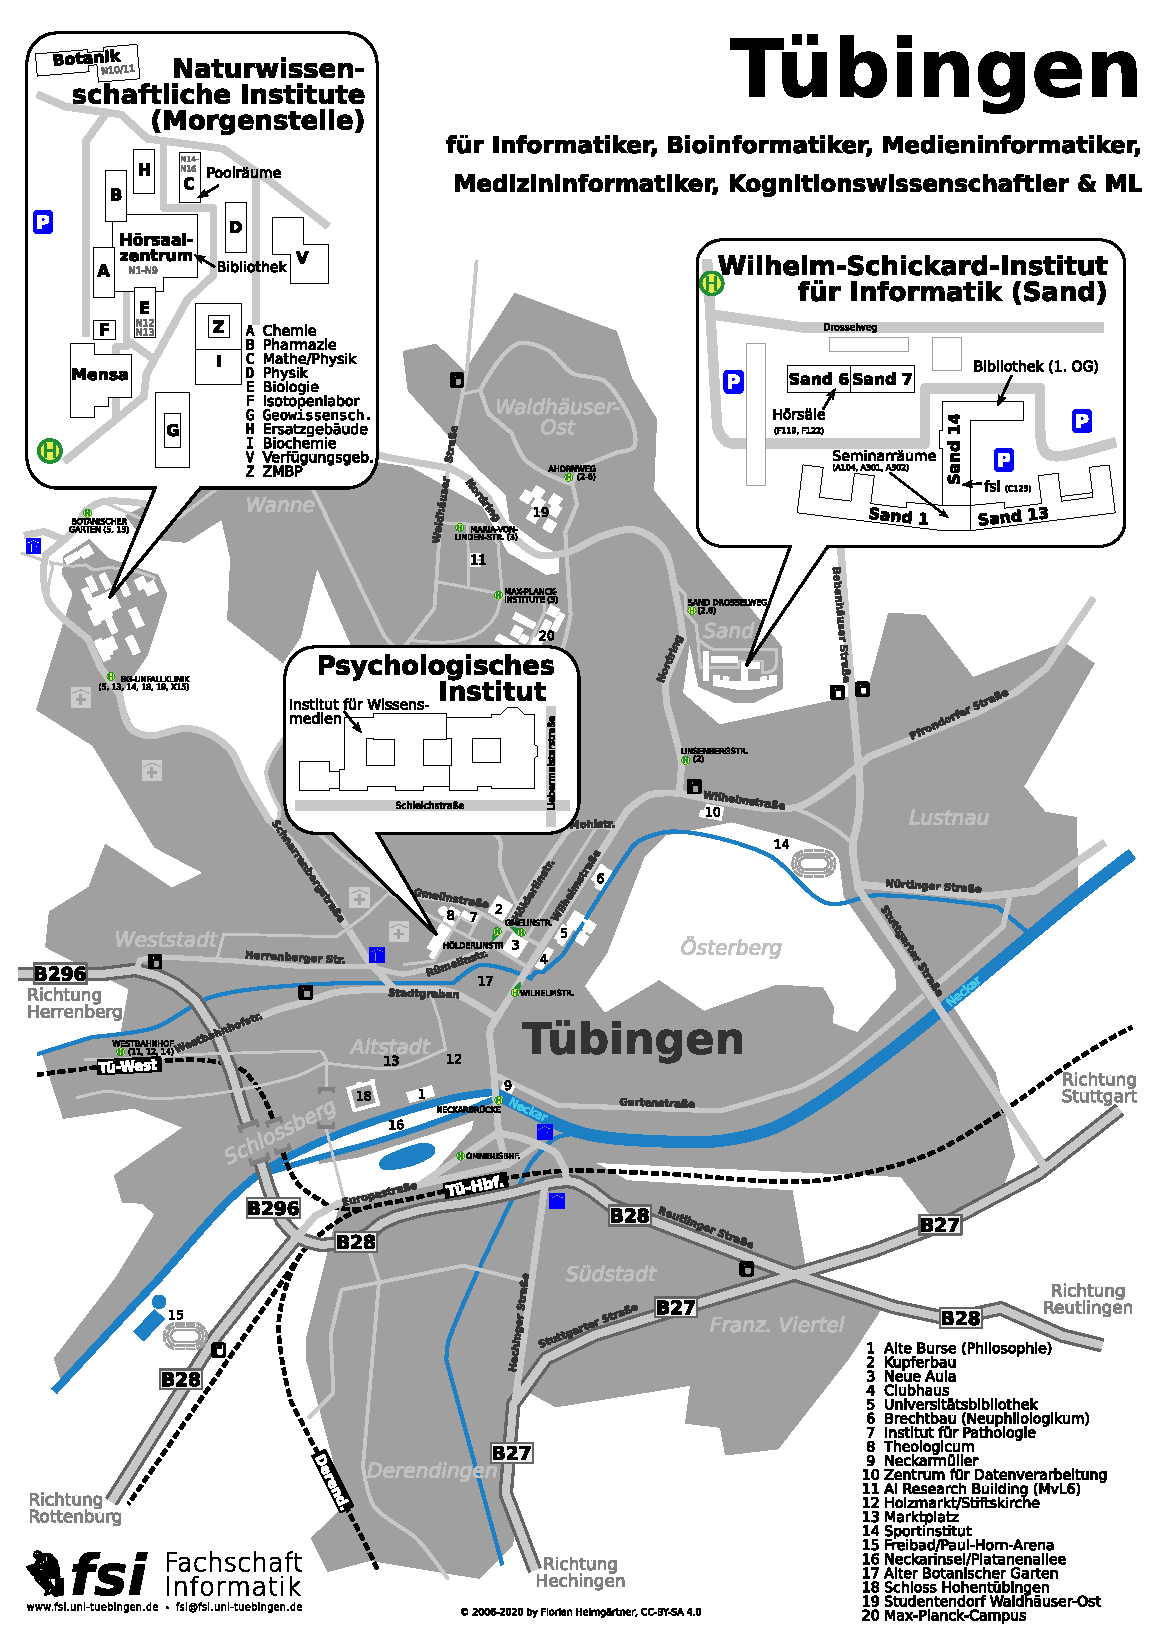
\includepdf[delta=5mm 5mm]{pdf/stadtplan.pdf}
  \end{letter}
\end{document}
